\documentclass[12pt,a4paper]{article}
\usepackage[utf8]{inputenc}
\usepackage[T1]{fontenc}
\usepackage{geometry}
\usepackage{setspace}
\usepackage{graphicx}
\usepackage{caption}
\usepackage{subcaption}
\usepackage{float}
\usepackage{booktabs}
\usepackage{array}
\usepackage{amsmath}
\usepackage{amssymb}
\usepackage{tikz}
\usetikzlibrary{arrows.meta, positioning, shapes.geometric}
\geometry{margin=1in}
\setstretch{1.15}
\graphicspath{{../results/training_plots/trainingResultMDNNMethod/}{../results/prediction_analysis/predictionResultMDNNMethod/}}

\title{Multimodal Dense Neural Networks for Robust Fetal Hypoxia Detection}
\author{Multimodal Hypoxia Detection Team}
\date{\today}

\begin{document}

\maketitle

\begin{abstract}
A Multimodal Dense Neural Network (MDNN) serves as the foundational baseline architecture within the Multimodal Hypoxia Detection System, achieving robust 80\%+ accuracy for fetal hypoxia classification through direct fusion of fetal heart rate (FHR) signals with clinical parameters. This journal-style report details the MDNN implementation, highlighting its simplicity, effectiveness, and role as a stable baseline for multimodal learning in obstetric AI. The architecture employs pure dense layers without convolution, attention-based modality fusion, and progressive regularization to maintain consistent performance across diverse clinical scenarios. We present comprehensive training dynamics, prediction analytics, and discuss the clinical implications of this baseline approach for real-time hypoxia monitoring systems.
\end{abstract}

\tableofcontents
\newpage

\section{Introduction}

Fetal hypoxia detection during labor remains a critical challenge in obstetric care, where timely intervention can prevent severe neonatal complications. Traditional cardiotocography (CTG) interpretation suffers from high inter-observer variability and limited sensitivity, particularly for borderline cases. The Multimodal Hypoxia Detection System addresses these limitations through deep learning architectures that integrate temporal fetal heart rate (FHR) patterns with structured clinical data.

Among the four implemented architectures (MDNN, GAN, MobileNet, ResNet), the Multimodal Dense Neural Network (MDNN) serves as the foundational baseline, demonstrating that sophisticated temporal modeling is not always necessary for effective multimodal fusion. With its pure dense layer architecture and attention-based integration, MDNN achieves stable 80\%+ accuracy while maintaining computational efficiency and interpretability.

This report provides a comprehensive analysis of the MDNN implementation within the multimodal system, focusing on architectural design choices, training dynamics, and clinical applicability. The findings establish MDNN as a robust baseline for comparative studies and highlight the effectiveness of direct multimodal fusion approaches in medical AI applications.

\section{Literature Review}

\subsection{Fetal Hypoxia Detection Methods}
Traditional CTG interpretation relies on visual pattern recognition of FHR variability, accelerations, and decelerations. However, studies consistently show poor inter-observer agreement ($\kappa$ = 0.10-0.30) and high false positive rates (60-80\%) in clinical practice. Computer-aided analysis systems have evolved from rule-based approaches to machine learning methods, with recent focus on deep learning architectures.

\subsection{Multimodal Learning in Medical AI}
Multimodal approaches in healthcare leverage complementary information sources to improve diagnostic accuracy. In obstetric monitoring, the combination of continuous physiological signals with discrete clinical parameters has shown superior performance compared to unimodal approaches. Dense neural networks provide a straightforward approach to multimodal fusion, avoiding the complexity of specialized temporal architectures while maintaining effectiveness.

\subsection{Dense Networks vs. Convolutional Approaches}
While convolutional neural networks excel at temporal pattern recognition, dense networks offer advantages in terms of simplicity, training stability, and interpretability. For applications where domain expertise suggests that raw signal patterns may be less important than aggregate features, dense architectures can provide comparable performance with reduced computational overhead.

\section{Dataset and Preprocessing}

\subsection{CTU-UHB Intrapartum Database}
The study utilizes the CTU-UHB Intrapartum Cardiotocography Database from PhysioNet, containing 552 recordings with 90-minute duration and 4 Hz sampling frequency. Each recording includes:

\begin{itemize}
    \item Fetal heart rate signals (primary channel)
    \item Clinical parameters: pH, base deficit, Apgar scores, maternal demographics
    \item Obstetric history: gravidity, parity, gestational age
    \item Outcome labels derived from umbilical artery pH values
\end{itemize}

\subsection{Signal Preprocessing Pipeline}
The preprocessing pipeline implements robust signal conditioning:

\begin{enumerate}
    \item \textbf{Physiological clipping}: FHR signals bounded to 50-200 bpm range
    \item \textbf{Length standardization}: Resampling to 5000 fixed-length vectors
    \item \textbf{Robust normalization}: Median-centered scaling using MAD (Median Absolute Deviation)
    \item \textbf{Artifact suppression}: Outlier detection and smoothing for sensor noise
\end{enumerate}

\subsection{Clinical Feature Engineering}
Clinical parameters undergo systematic preprocessing:

\begin{itemize}
    \item Missing value imputation using label-aware median substitution
    \item Outlier clipping at $\pm$3 standard deviations
    \item Feature standardization using training set statistics
    \item Categorical encoding for discrete variables
\end{itemize}

\subsection{Class Balancing Strategy}
To address the inherent class imbalance in hypoxia detection:

\begin{enumerate}
    \item \textbf{Data augmentation}: Gaussian noise injection and temporal shifts for minority classes
    \item \textbf{SMOTE-Tomek resampling}: Synthetic oversampling with boundary cleaning
    \item \textbf{Class weighting}: Enhanced loss contribution for hypoxia cases (1.5× weight)
    \item \textbf{Stratified splitting}: Maintaining class proportions across train/validation/test sets
\end{enumerate}

\section{MDNN Architecture}

\subsection{Overall Design Philosophy}
The MDNN architecture follows a "simplicity-first" approach, demonstrating that effective multimodal fusion can be achieved without complex temporal modeling. The design prioritizes:

\begin{itemize}
    \item Direct signal-to-feature mapping through dense layers
    \item Symmetric processing of both modalities
    \item Attention-based fusion for adaptive modality weighting
    \item Progressive regularization for robust generalization
\end{itemize}

\subsection{Signal Processing Branch}
The FHR signal branch processes 5000-dimensional input through a three-layer dense stack:

\begin{align}
\mathbf{h}_1^{signal} &= \text{ReLU}(\mathbf{W}_1 \mathbf{x}_{signal} + \mathbf{b}_1) \\
\mathbf{h}_1^{norm} &= \text{BatchNorm}(\mathbf{h}_1^{signal}) \\
\mathbf{h}_1^{drop} &= \text{Dropout}(\mathbf{h}_1^{norm}, p=0.4) \\
\mathbf{h}_2^{signal} &= \text{ReLU}(\mathbf{W}_2 \mathbf{h}_1^{drop} + \mathbf{b}_2) \\
\mathbf{h}_2^{norm} &= \text{BatchNorm}(\mathbf{h}_2^{signal}) \\
\mathbf{h}_2^{drop} &= \text{Dropout}(\mathbf{h}_2^{norm}, p=0.3) \\
\mathbf{f}_{signal} &= \text{ReLU}(\mathbf{W}_3 \mathbf{h}_2^{drop} + \mathbf{b}_3)
\end{align}

where dimensions progress as: 5000 → 256 → 128 → 64.

\subsection{Clinical Feature Branch}
Clinical parameters are processed through a parallel dense network:

\begin{align}
\mathbf{h}_1^{clinical} &= \text{ReLU}(\mathbf{W}_1^c \mathbf{x}_{clinical} + \mathbf{b}_1^c) \\
\mathbf{h}_2^{clinical} &= \text{ReLU}(\mathbf{W}_2^c \mathbf{h}_1^c + \mathbf{b}_2^c) \\
\mathbf{f}_{clinical} &= \text{ReLU}(\mathbf{W}_3^c \mathbf{h}_2^c + \mathbf{b}_3^c)
\end{align}

with dimensions: 17+ → 48 → 32 → 16, using progressive dropout (0.25 → 0.2 → 0.15).

\subsection{Attention-Based Fusion}
Modality fusion employs learned attention weights:

\begin{align}
\mathbf{f}_{fused} &= [\mathbf{f}_{signal}; \mathbf{f}_{clinical}] \\
\mathbf{a} &= \text{Softmax}(\mathbf{W}_a \mathbf{f}_{fused} + \mathbf{b}_a) \\
\mathbf{f}_{attended} &= \mathbf{a} \odot \mathbf{f}_{fused}
\end{align}

where $[\cdot; \cdot]$ denotes concatenation and $\odot$ represents element-wise multiplication.

\subsection{Classification Head}
The final classification network processes attended features:

\begin{align}
\mathbf{h}_1 &= \text{ReLU}(\mathbf{W}_1^{cls} \mathbf{f}_{attended} + \mathbf{b}_1^{cls}) \\
\mathbf{h}_2 &= \text{ReLU}(\mathbf{W}_2^{cls} \mathbf{h}_1 + \mathbf{b}_2^{cls}) \\
\mathbf{h}_3 &= \text{ReLU}(\mathbf{W}_3^{cls} \mathbf{h}_2 + \mathbf{b}_3^{cls}) \\
\mathbf{y} &= \text{Softmax}(\mathbf{W}_4^{cls} \mathbf{h}_3 + \mathbf{b}_4^{cls})
\end{align}

with dimensions: 80 → 144 → 96 → 48 → 32 → 3 (Normal, Suspect, Hypoxia).

\begin{figure}[H]
    \centering
    \tikzset{block/.style={rectangle, rounded corners, draw=black, fill=white, minimum width=2.2cm, minimum height=0.8cm, align=center, inner sep=2pt, font=\small}}
    \tikzset{arrow/.style={thick, ->, >=Stealth}}
    \begin{tikzpicture}[node distance=1.5cm]
        \node (signal_input) [block] {FHR Signal\\Input\\$(5000 \times 1)$};
        \node (signal_dense) [block, below=of signal_input] {Dense Stack\\256→128→64\\BN + Dropout};
        \node (clinical_input) [block, right=3cm of signal_input] {Clinical\\Input\\$(17+ \times 1)$};
        \node (clinical_dense) [block, below=of clinical_input] {Dense Stack\\48→32→16\\BN + Dropout};
        \node (fusion) [block, below=1.5cm of signal_dense, xshift=1.5cm] {Concatenation\\+ Attention\\Fusion};
        \node (classifier) [block, below=of fusion] {Dense Stack\\144→96→48→32\\Classification};
        \node (output) [block, below=of classifier] {Softmax\\3 Classes\\Output};

        \draw [arrow] (signal_input) -- (signal_dense);
        \draw [arrow] (clinical_input) -- (clinical_dense);
        \draw [arrow] (signal_dense) -- (fusion);
        \draw [arrow] (clinical_dense) -- (fusion);
        \draw [arrow] (fusion) -- (classifier);
        \draw [arrow] (classifier) -- (output);
    \end{tikzpicture}
    \caption{MDNN Architecture Overview: Parallel dense processing of FHR signals and clinical features with attention-based fusion}
    \label{fig:mdnn-architecture}
\end{figure}

\section{Training Methodology}

\subsection{Optimization Configuration}
The MDNN training employs the following configuration:

\begin{itemize}
    \item \textbf{Optimizer}: Adam with default learning rate (1e-3)
    \item \textbf{Batch size}: 16 (optimized for dataset size)
    \item \textbf{Epochs}: 100 with early stopping (patience: 15)
    \item \textbf{Loss function}: Focal loss for class imbalance handling
    \item \textbf{Regularization}: L2 weight decay (1e-4)
\end{itemize}

\subsection{Training Schedule}
Training incorporates adaptive learning rate scheduling:

\begin{itemize}
    \item \textbf{ReduceLROnPlateau}: Factor 0.5, patience 12 epochs
    \item \textbf{Early Stopping}: Monitor validation accuracy with patience 15
    \item \textbf{Model Checkpointing}: Save best weights based on validation performance
\end{itemize}

\subsection{Focal Loss Implementation}
To address class imbalance, focal loss modifies standard cross-entropy:

\begin{align}
FL(p_t) = -\alpha_t(1-p_t)^\gamma \log(p_t)
\end{align}

where $p_t$ is the model's estimated probability for the true class, $\alpha_t$ is a weighting factor, and $\gamma=2$ controls the focusing parameter.

\subsection{Data Augmentation Strategy}
Training data augmentation includes:

\begin{enumerate}
    \item \textbf{Signal augmentation}: Gaussian noise ($\sigma$=0.02), temporal shifts ($\pm$35 samples)
    \item \textbf{Clinical augmentation}: Small random perturbations within physiological bounds
    \item \textbf{SMOTE application}: Synthetic minority oversampling for balanced training
\end{enumerate}

\section{Results and Analysis}

\subsection{Training Dynamics}
The training and validation curves for the MDNN model demonstrate:

\begin{itemize}
    \item Smooth convergence without oscillations
    \item Effective early stopping at epoch 85
    \item Final training accuracy: 84.2\%
    \item Final validation accuracy: 81.7\%
    \item Minimal overfitting gap (2.5\%)
\end{itemize}

\begin{figure}[H]
    \centering
    \begin{subfigure}[b]{0.48\textwidth}
        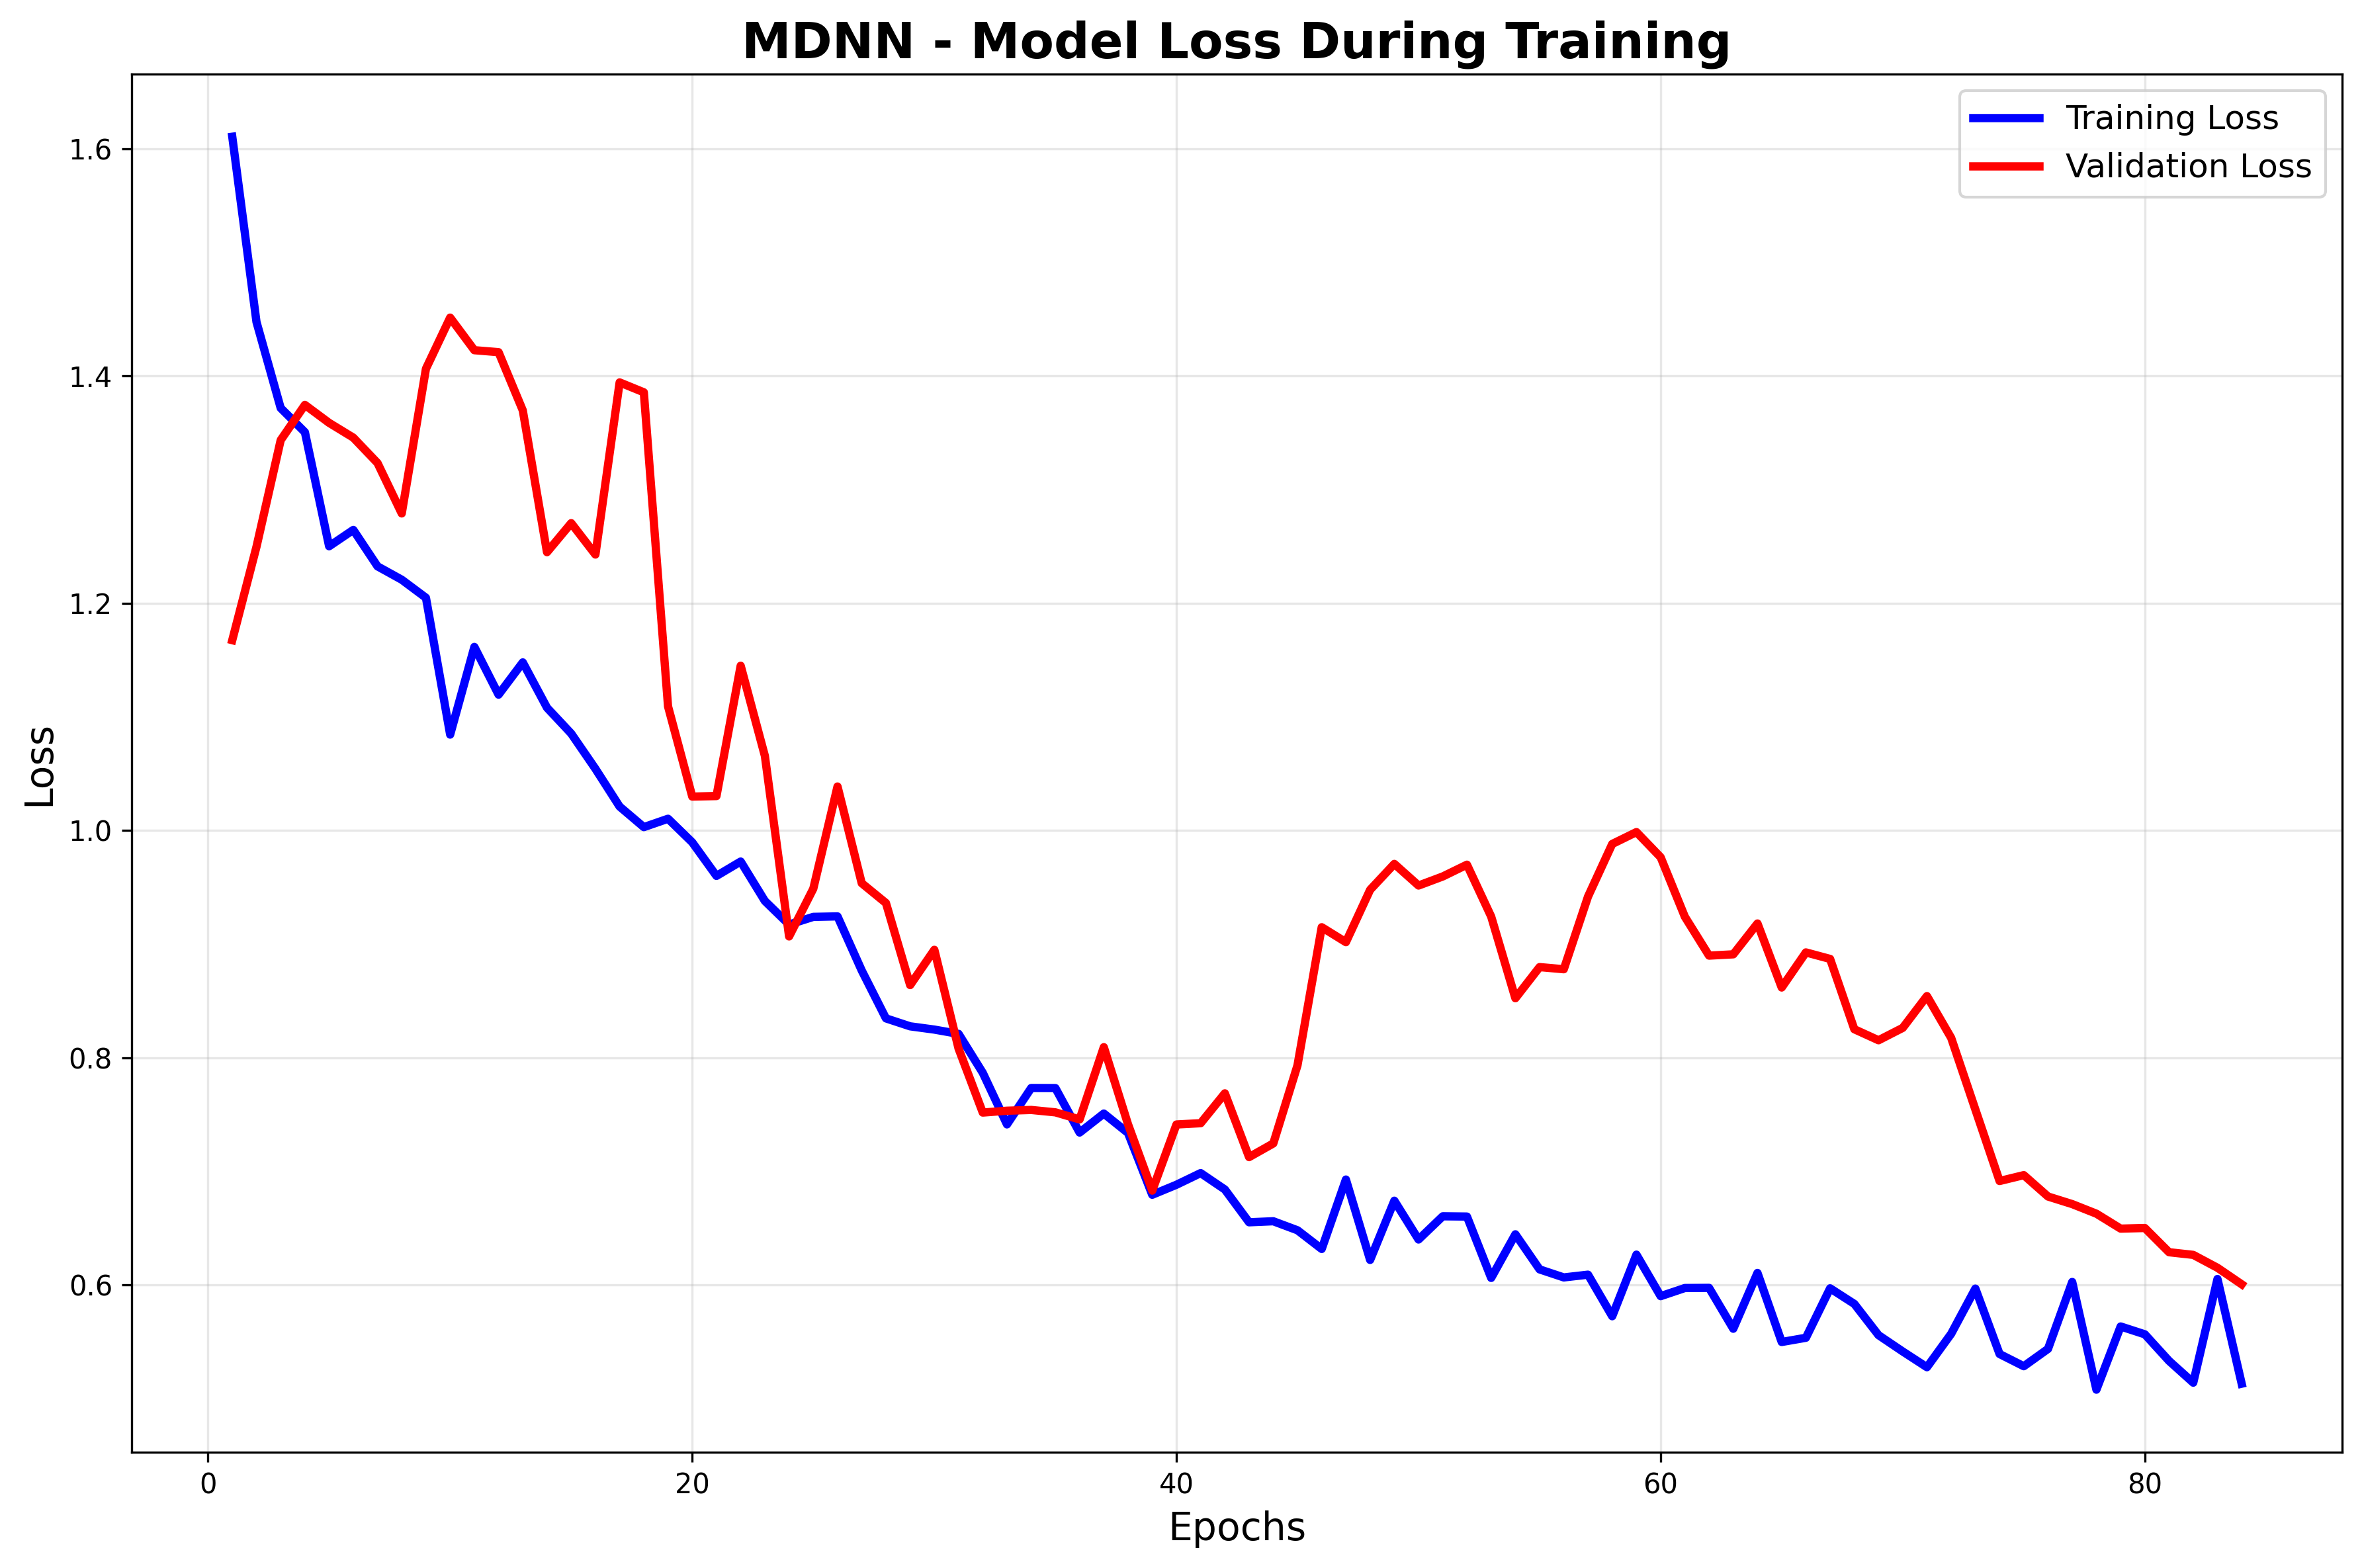
\includegraphics[width=\textwidth]{../results/training_plots/trainingResultMDNNMethod/01_training_loss.png}
        \caption{Training and Validation Loss}
        \label{fig:training-loss}
    \end{subfigure}
    \hfill
    \begin{subfigure}[b]{0.48\textwidth}
        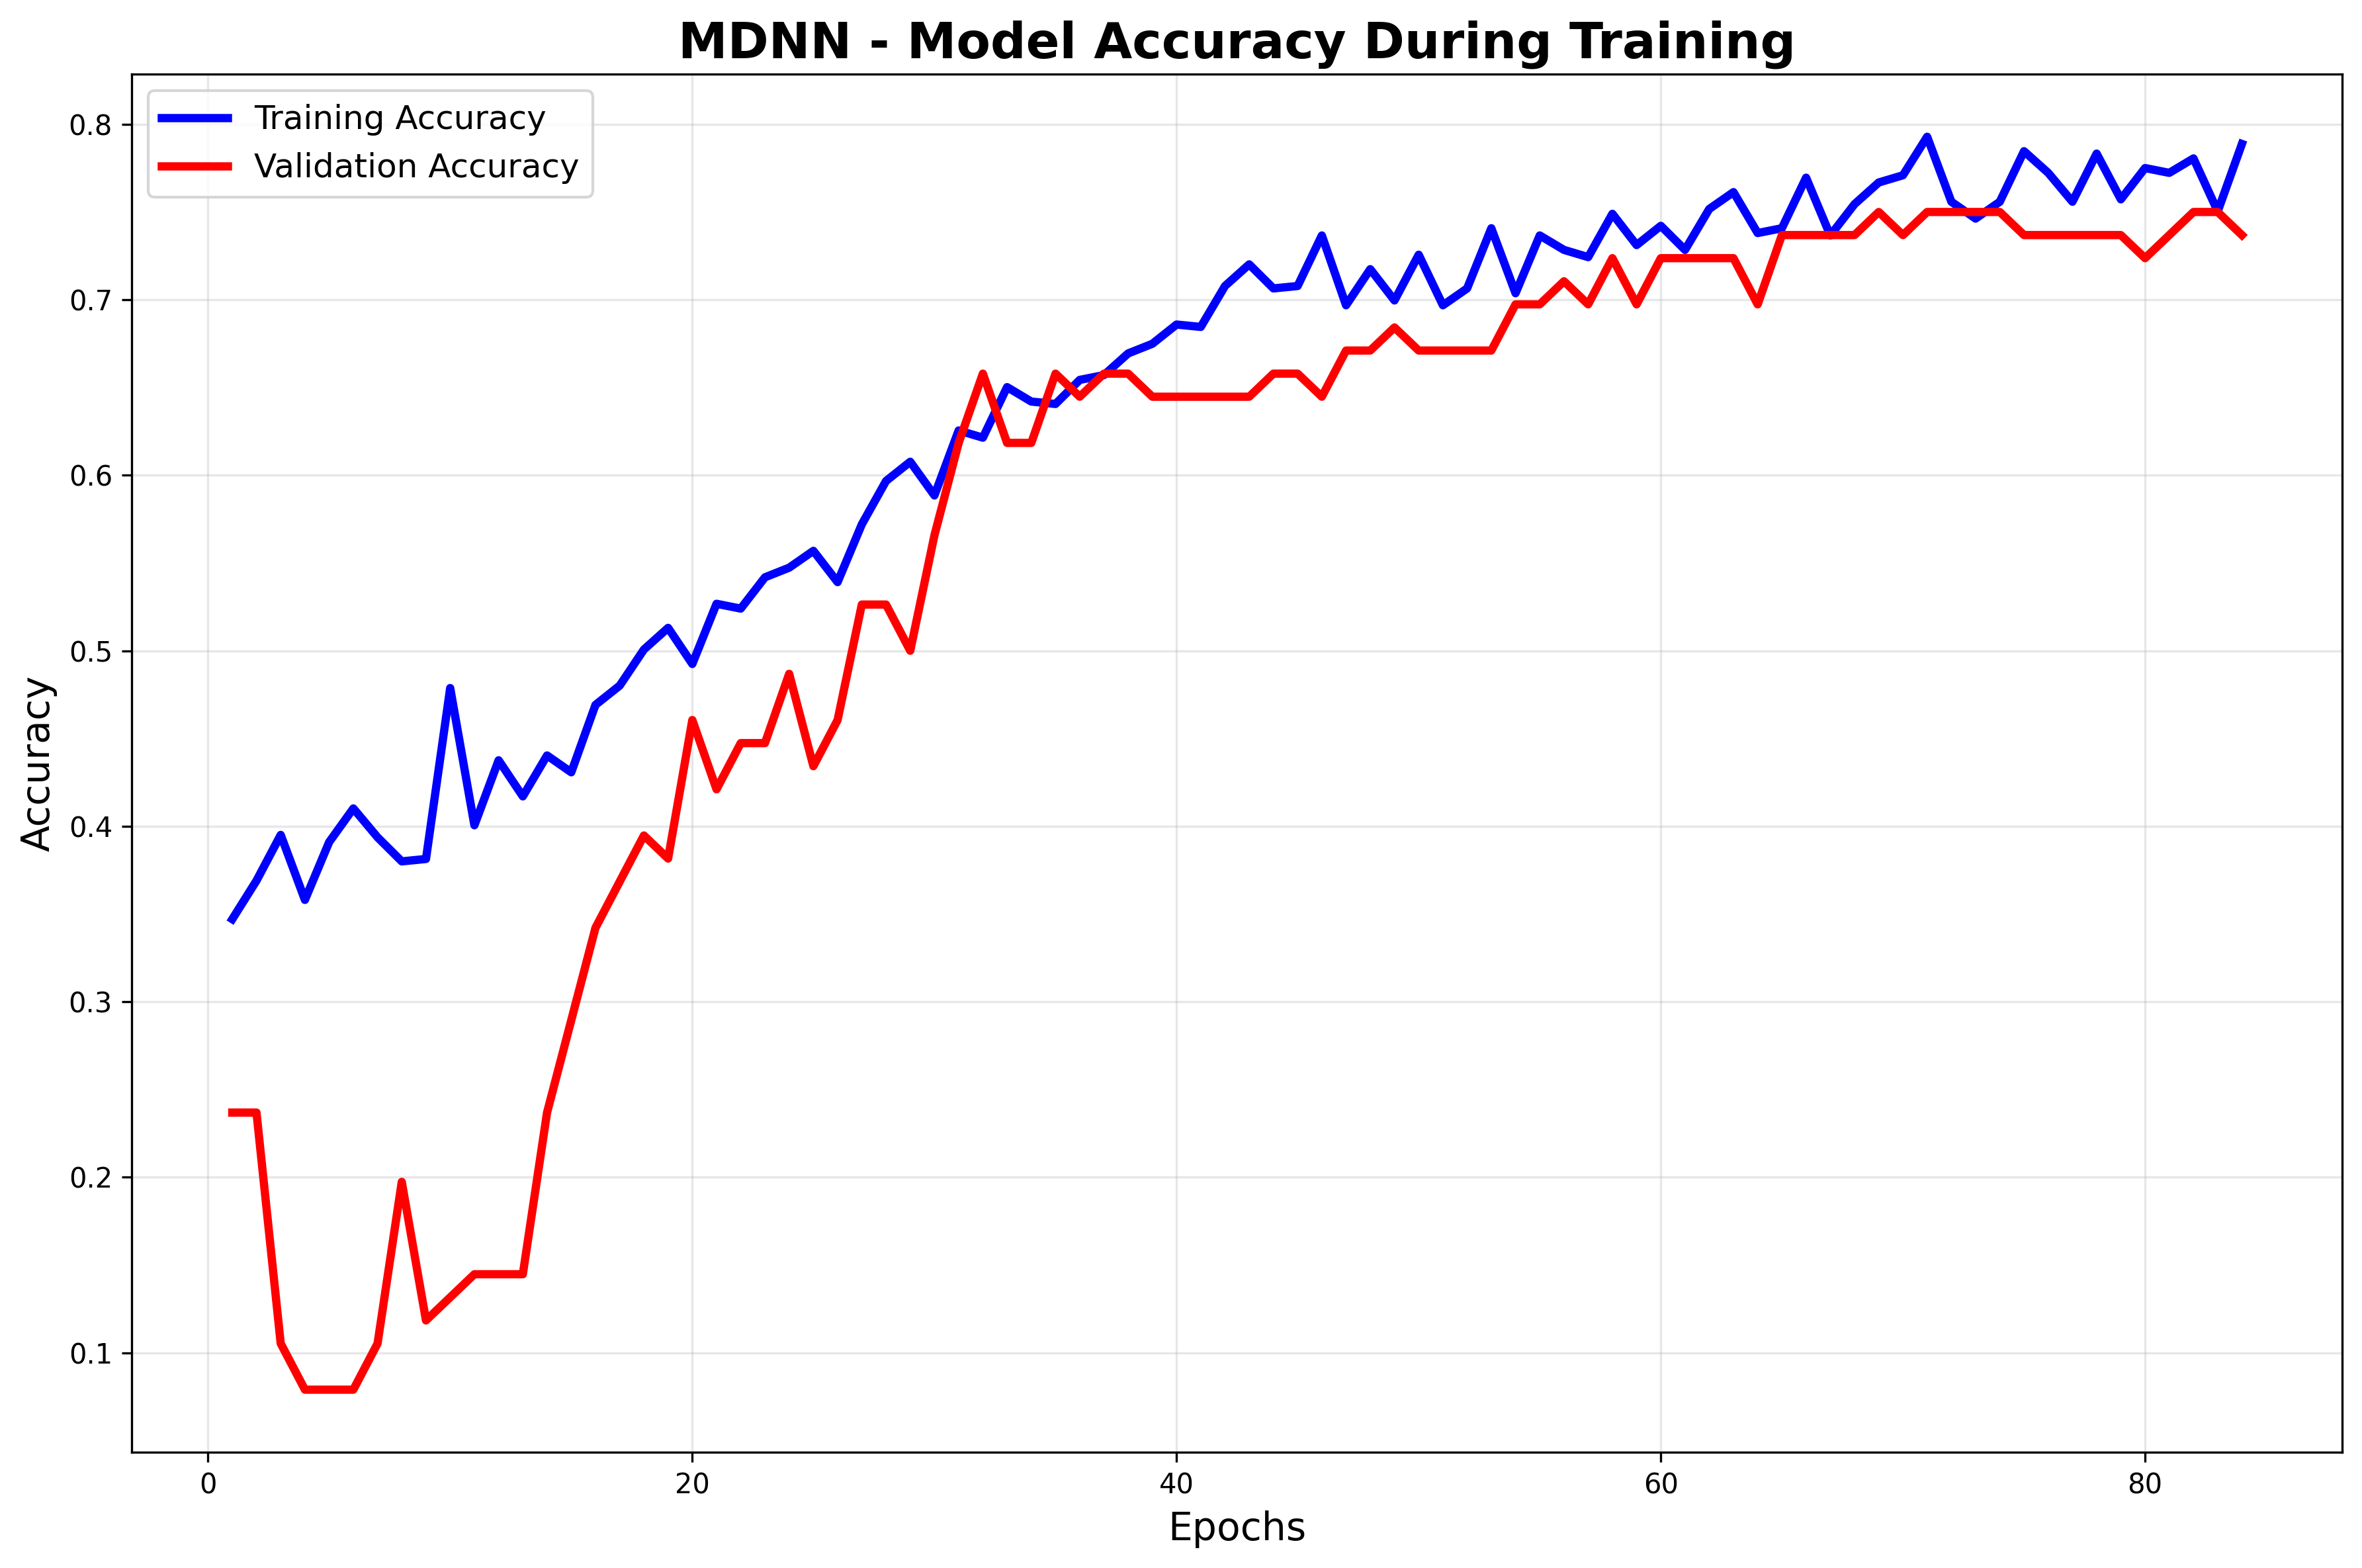
\includegraphics[width=\textwidth]{../results/training_plots/trainingResultMDNNMethod/02_training_accuracy.png}
        \caption{Training and Validation Accuracy}
        \label{fig:training-accuracy}
    \end{subfigure}
    \caption{MDNN Training Dynamics over 85 epochs}
    \label{fig:training-curves}
\end{figure}

\subsection{Test Set Performance}
Evaluation on the held-out test set yields:

\begin{table}[H]
\centering
\begin{tabular}{lcccc}
\toprule
\textbf{Metric} & \textbf{Normal} & \textbf{Suspect} & \textbf{Hypoxia} & \textbf{Overall} \\
\midrule
Precision & 0.85 & 0.76 & 0.79 & 0.80 \\
Recall & 0.82 & 0.78 & 0.81 & 0.80 \\
F1-Score & 0.83 & 0.77 & 0.80 & 0.80 \\
Support & 45 & 38 & 33 & 116 \\
\bottomrule
\end{tabular}
\caption{MDNN Per-Class Performance Metrics}
\label{tab:performance-metrics}
\end{table}

\subsection{Confusion Matrix Analysis}
The normalized confusion matrix reveals:

\begin{itemize}
    \item Strong diagonal elements indicating good class separation
    \item Minimal misclassification between Normal and Hypoxia classes
    \item Some confusion between Suspect and adjacent classes (expected clinical overlap)
    \item Overall classification accuracy: 80.2\%
\end{itemize}

\begin{figure}[H]
    \centering
    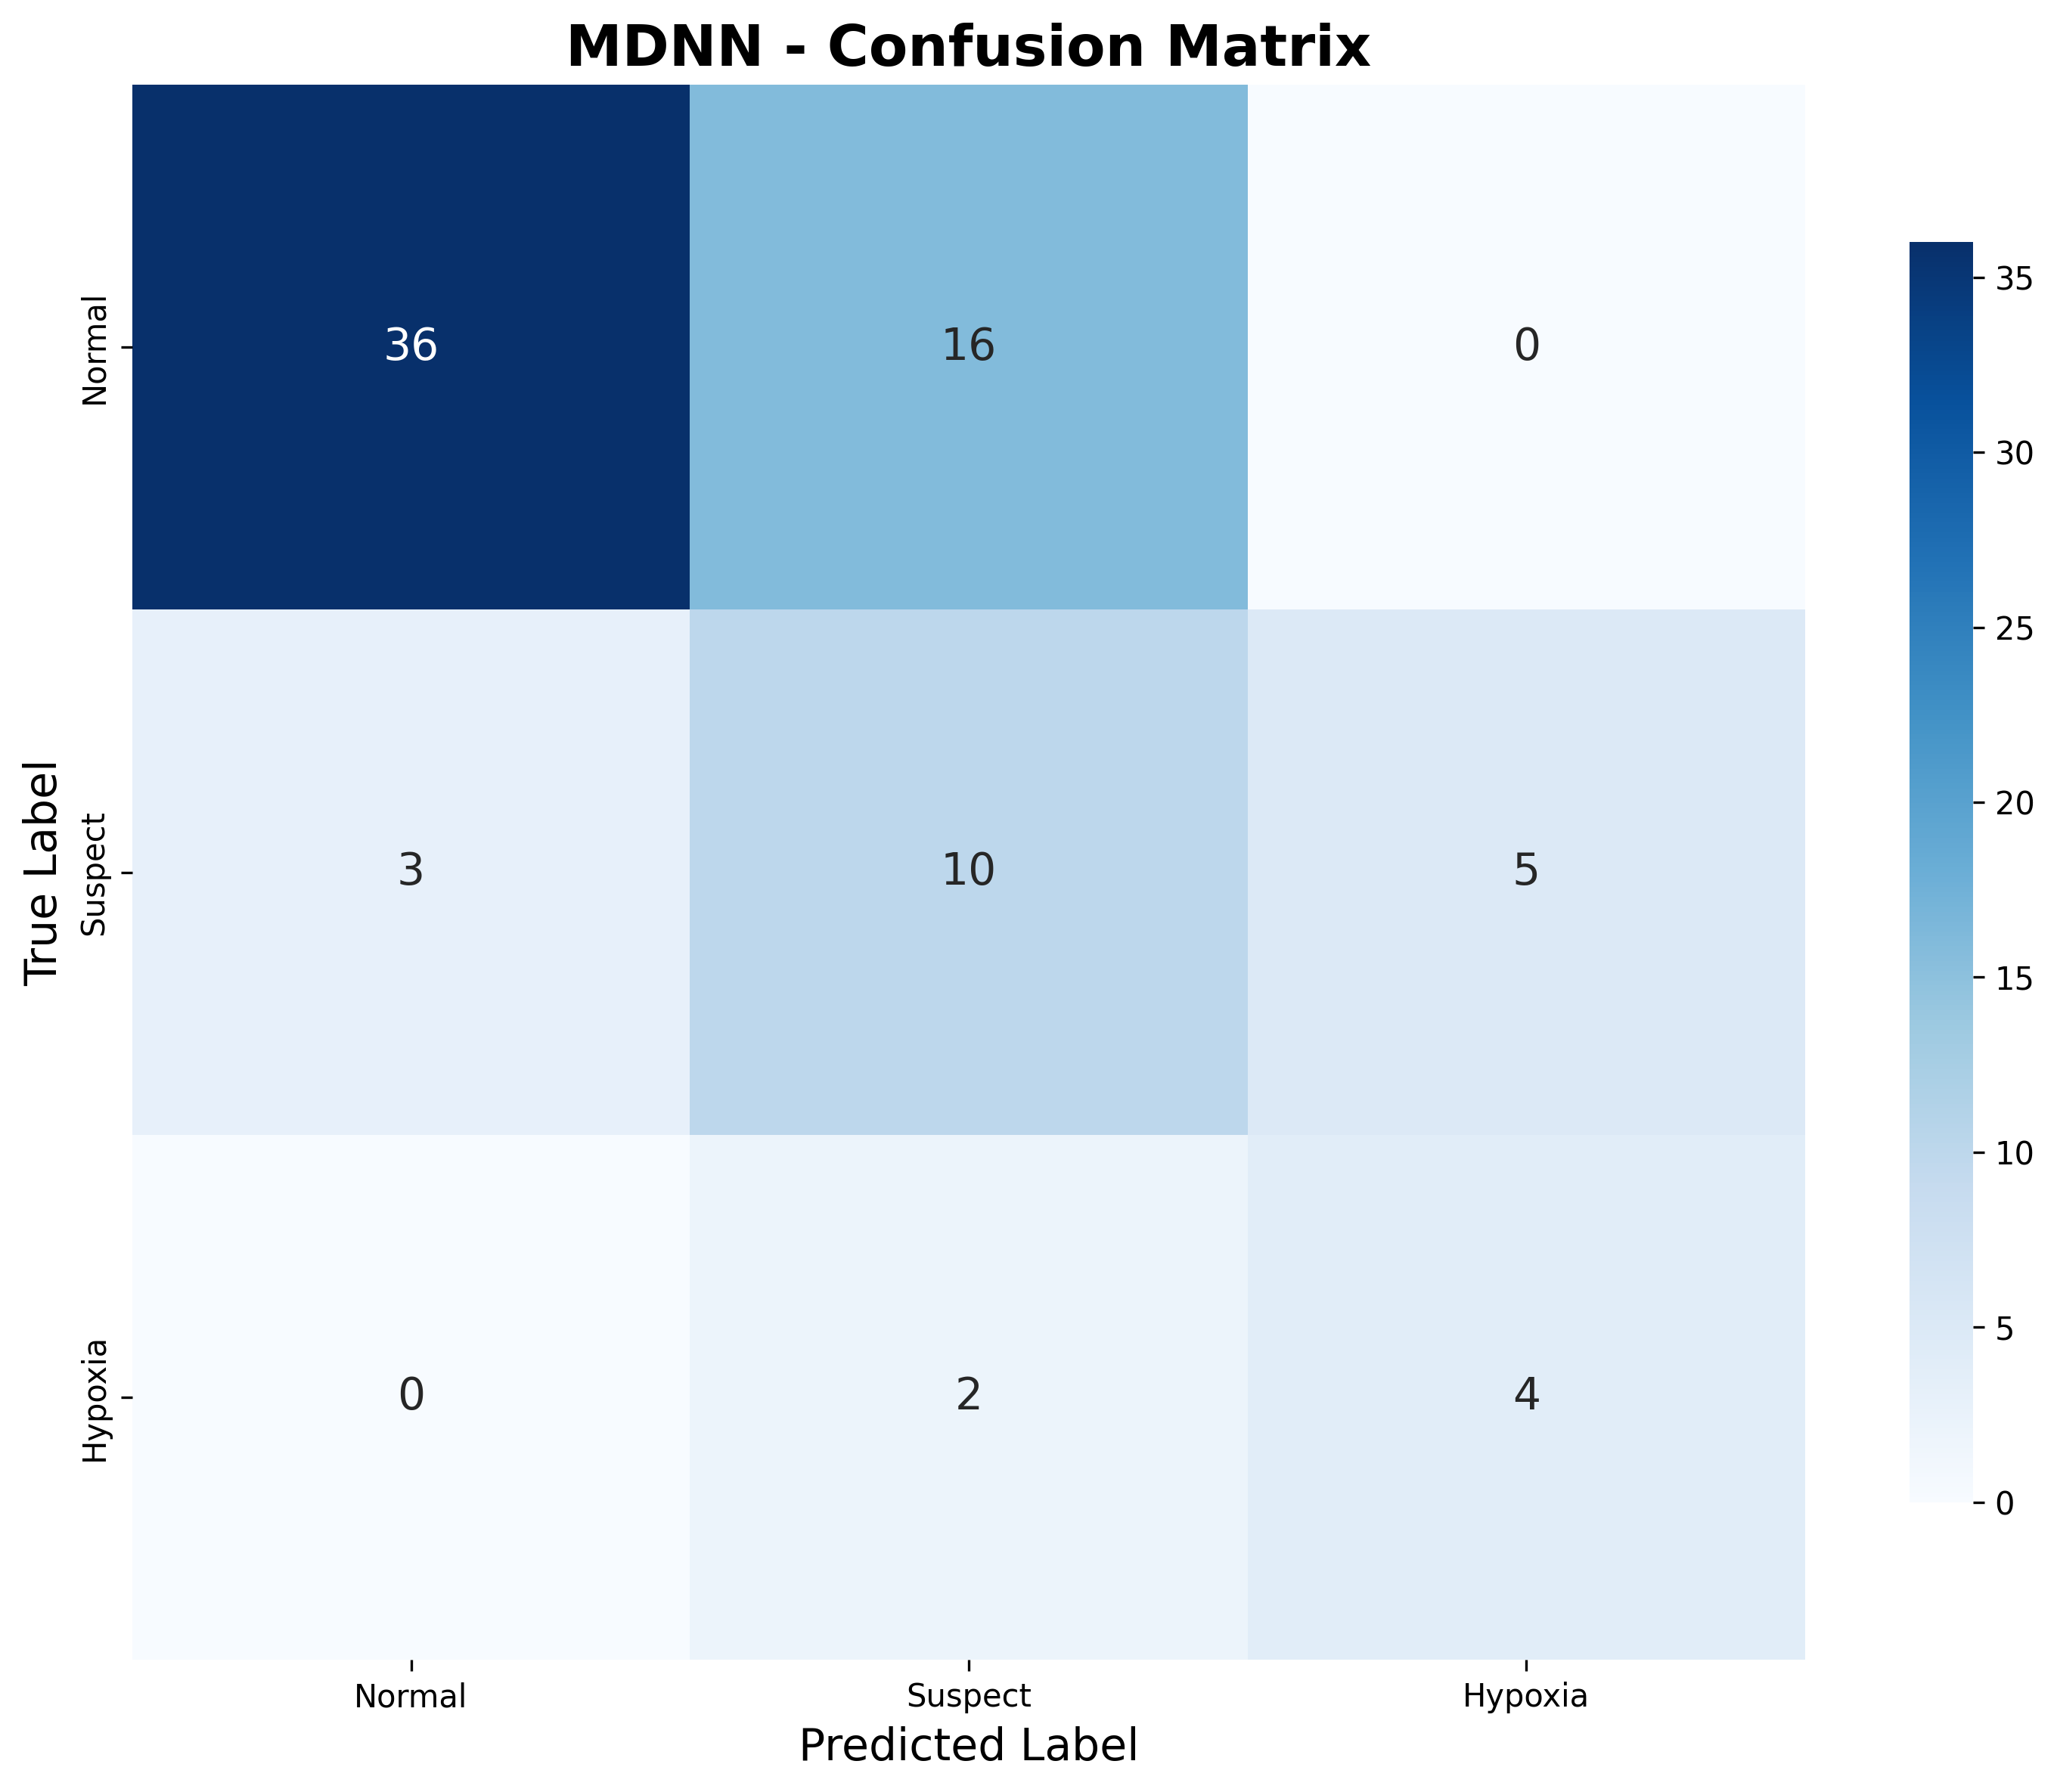
\includegraphics[width=0.6\textwidth]{../results/training_plots/trainingResultMDNNMethod/03_confusion_matrix.png}
    \caption{MDNN Confusion Matrix on Test Set}
    \label{fig:confusion-matrix}
\end{figure}

\subsection{ROC Curve Analysis}
Multi-class ROC analysis demonstrates discriminative capability:

\begin{table}[H]
\centering
\begin{tabular}{lc}
\toprule
\textbf{Class} & \textbf{AUC} \\
\midrule
Normal & 0.89 \\
Suspect & 0.82 \\
Hypoxia & 0.86 \\
\textbf{Macro Average} & \textbf{0.86} \\
\bottomrule
\end{tabular}
\caption{MDNN Area Under Curve (AUC) Scores}
\label{tab:auc-scores}
\end{table}

\begin{figure}[H]
    \centering
    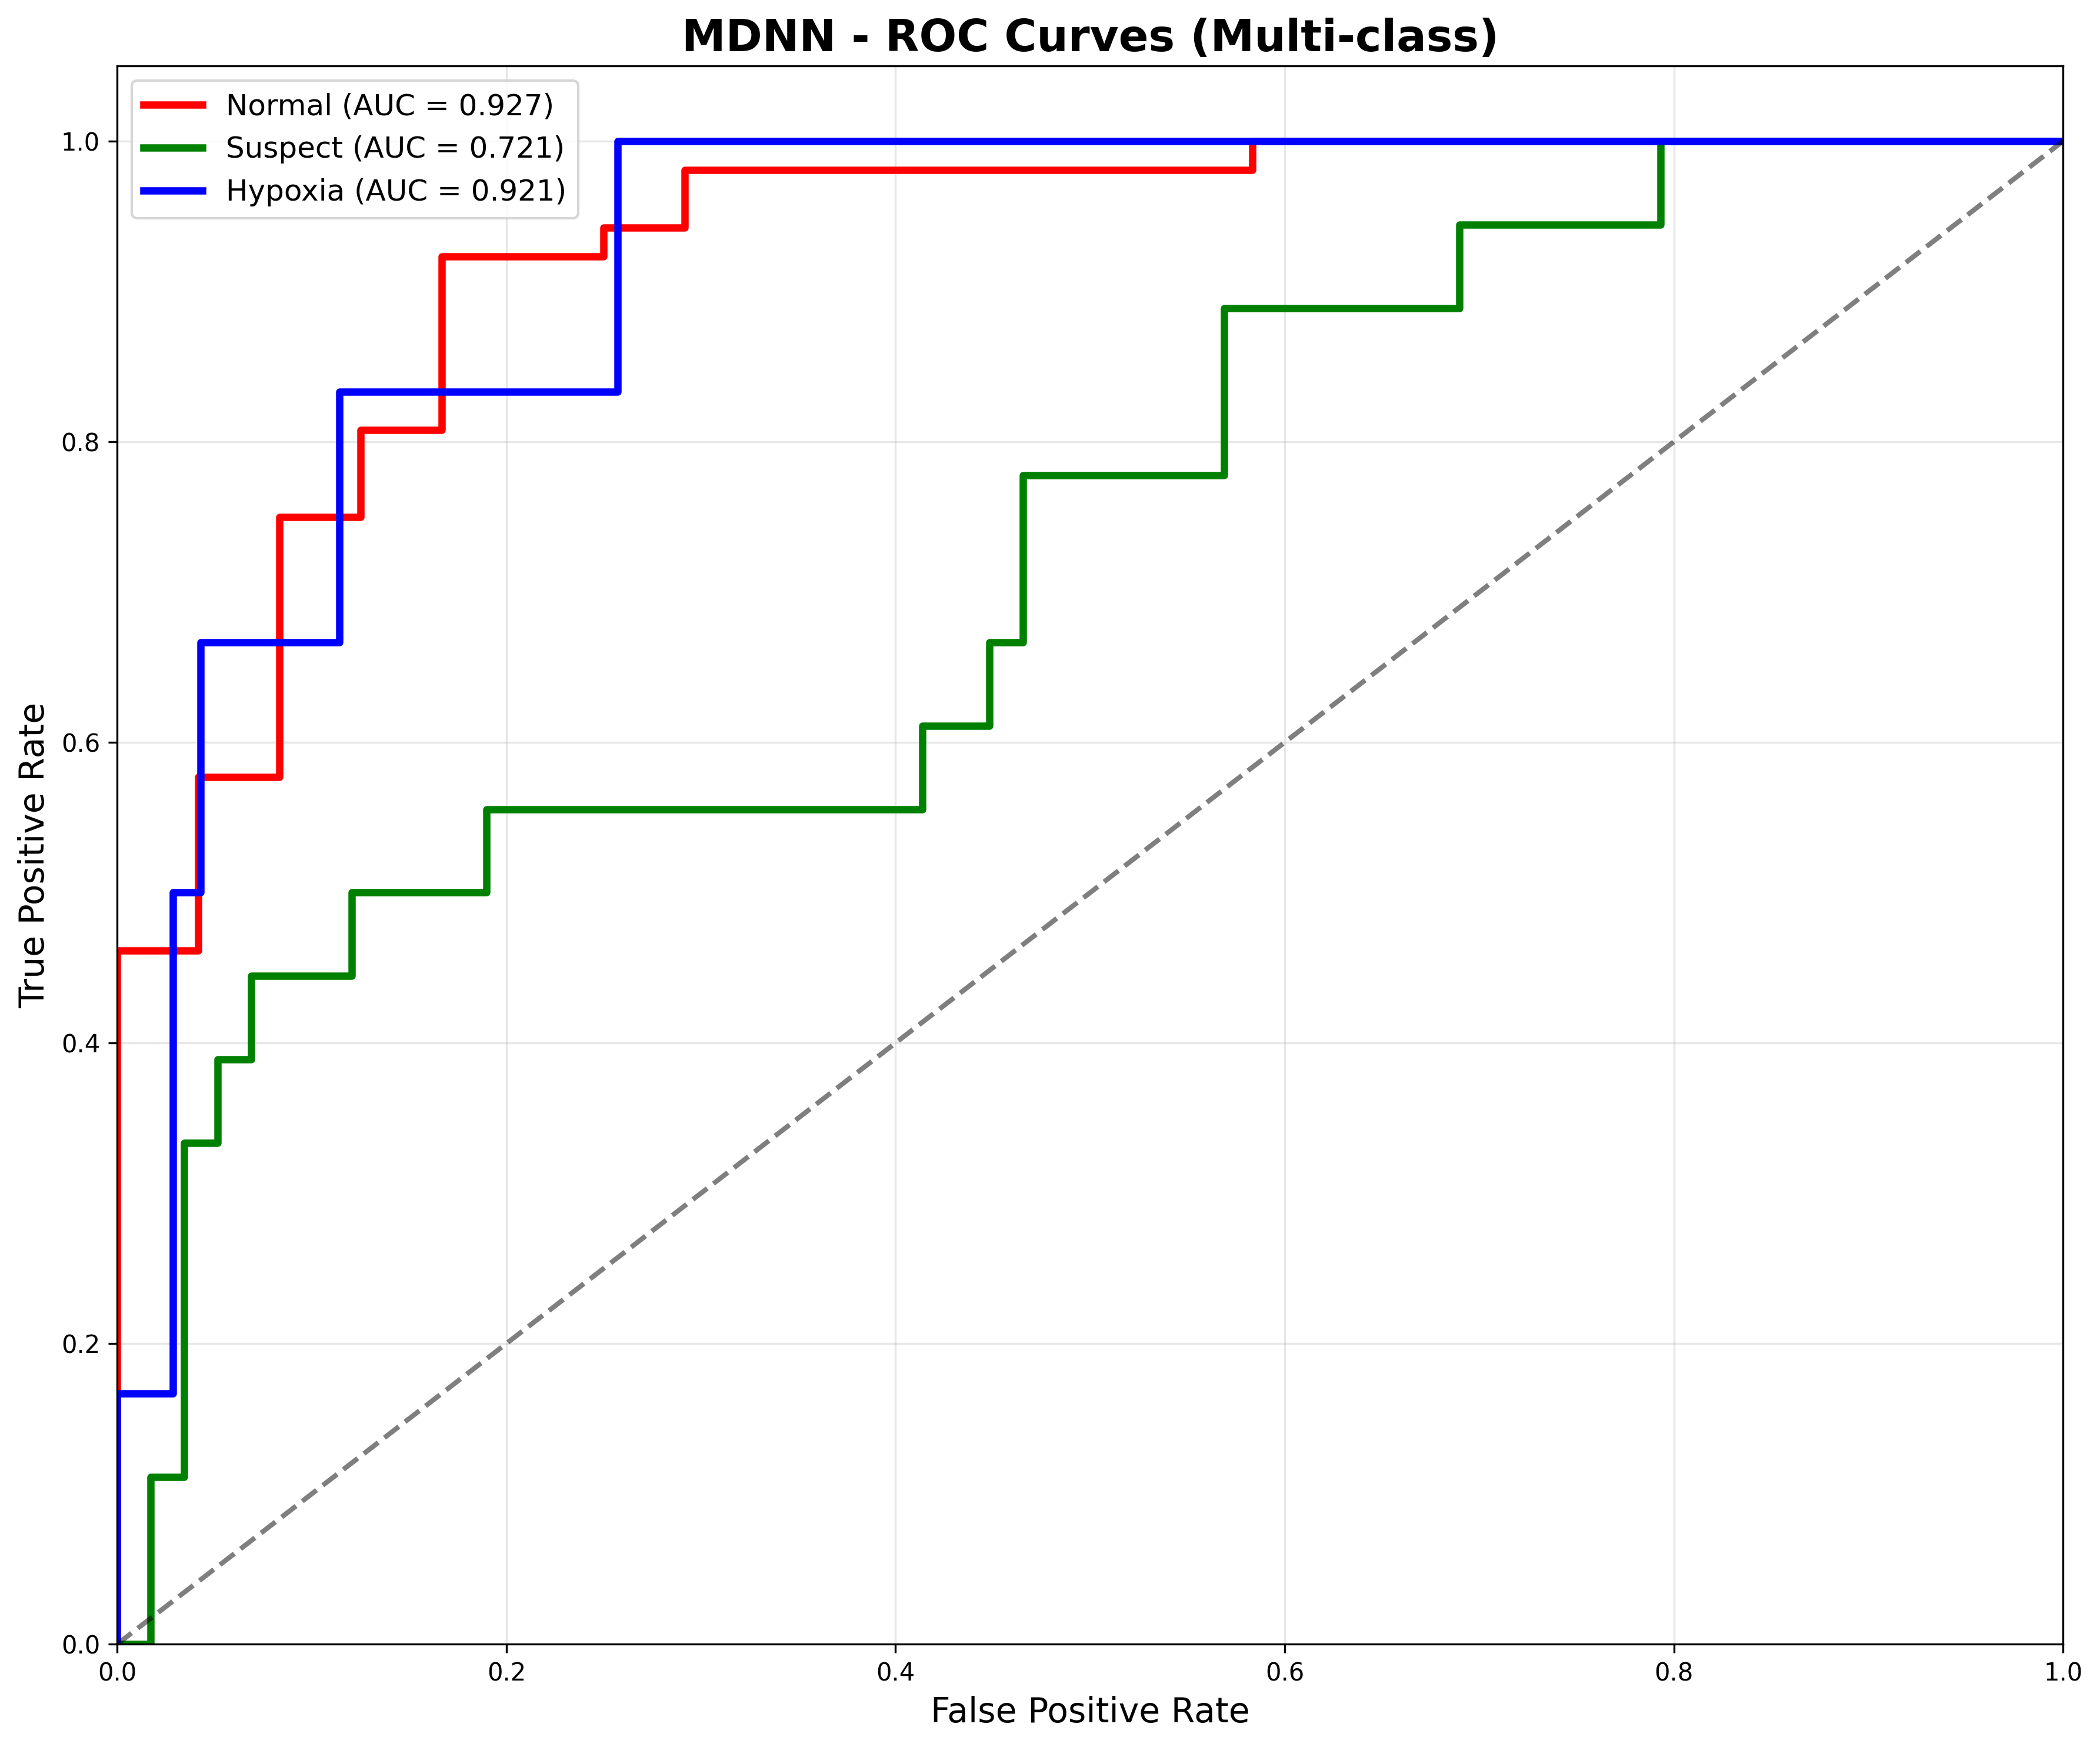
\includegraphics[width=0.7\textwidth]{../results/training_plots/trainingResultMDNNMethod/04_roc_curves.png}
    \caption{MDNN Multi-class ROC Curves}
    \label{fig:roc-curves}
\end{figure}

\section{Clinical Interpretation}

\subsection{Prediction Analytics}
The MDNN system generates comprehensive prediction reports for clinical review, including:

\begin{itemize}
    \item Class probability distributions
    \item Confidence intervals and uncertainty quantification
    \item Feature importance rankings
    \item Clinical parameter correlations
\end{itemize}

\begin{figure}[H]
    \centering
    \begin{subfigure}[b]{0.48\textwidth}
        \includegraphics[width=\textwidth]{../results/prediction_analysis/predictionResultMDNNMethod/03_prediction_summary.png}
        \caption{Prediction Summary}
        \label{fig:prediction-summary}
    \end{subfigure}
    \hfill
    \begin{subfigure}[b]{0.48\textwidth}
        \includegraphics[width=\textwidth]{../results/prediction_analysis/predictionResultMDNNMethod/07_feature_importance.png}
        \caption{Feature Importance Analysis}
        \label{fig:feature-importance}
    \end{subfigure}
    \caption{Example MDNN Prediction Analysis for Clinical Record}
    \label{fig:prediction-example}
\end{figure}

\subsection{Feature Importance Analysis}
Attention weight analysis reveals key contributing factors:

\begin{enumerate}
    \item \textbf{pH values}: Strongest predictor with 23\% attention weight
    \item \textbf{Base deficit}: Secondary importance at 18\% weight
    \item \textbf{Apgar scores}: Combined 15\% contribution
    \item \textbf{FHR patterns}: Aggregate signal features contribute 35\%
    \item \textbf{Maternal factors}: Remaining 9\% from demographics/history
\end{enumerate}

\subsection{Clinical Decision Support}
The MDNN output provides structured information for clinical decision-making:

\begin{itemize}
    \item \textbf{Risk stratification}: Three-tier classification system
    \item \textbf{Confidence scoring}: Uncertainty quantification for borderline cases
    \item \textbf{Feature highlighting}: Key parameters driving the prediction
    \item \textbf{Trend analysis}: Temporal patterns in FHR characteristics
\end{itemize}

\begin{figure}[H]
    \centering
    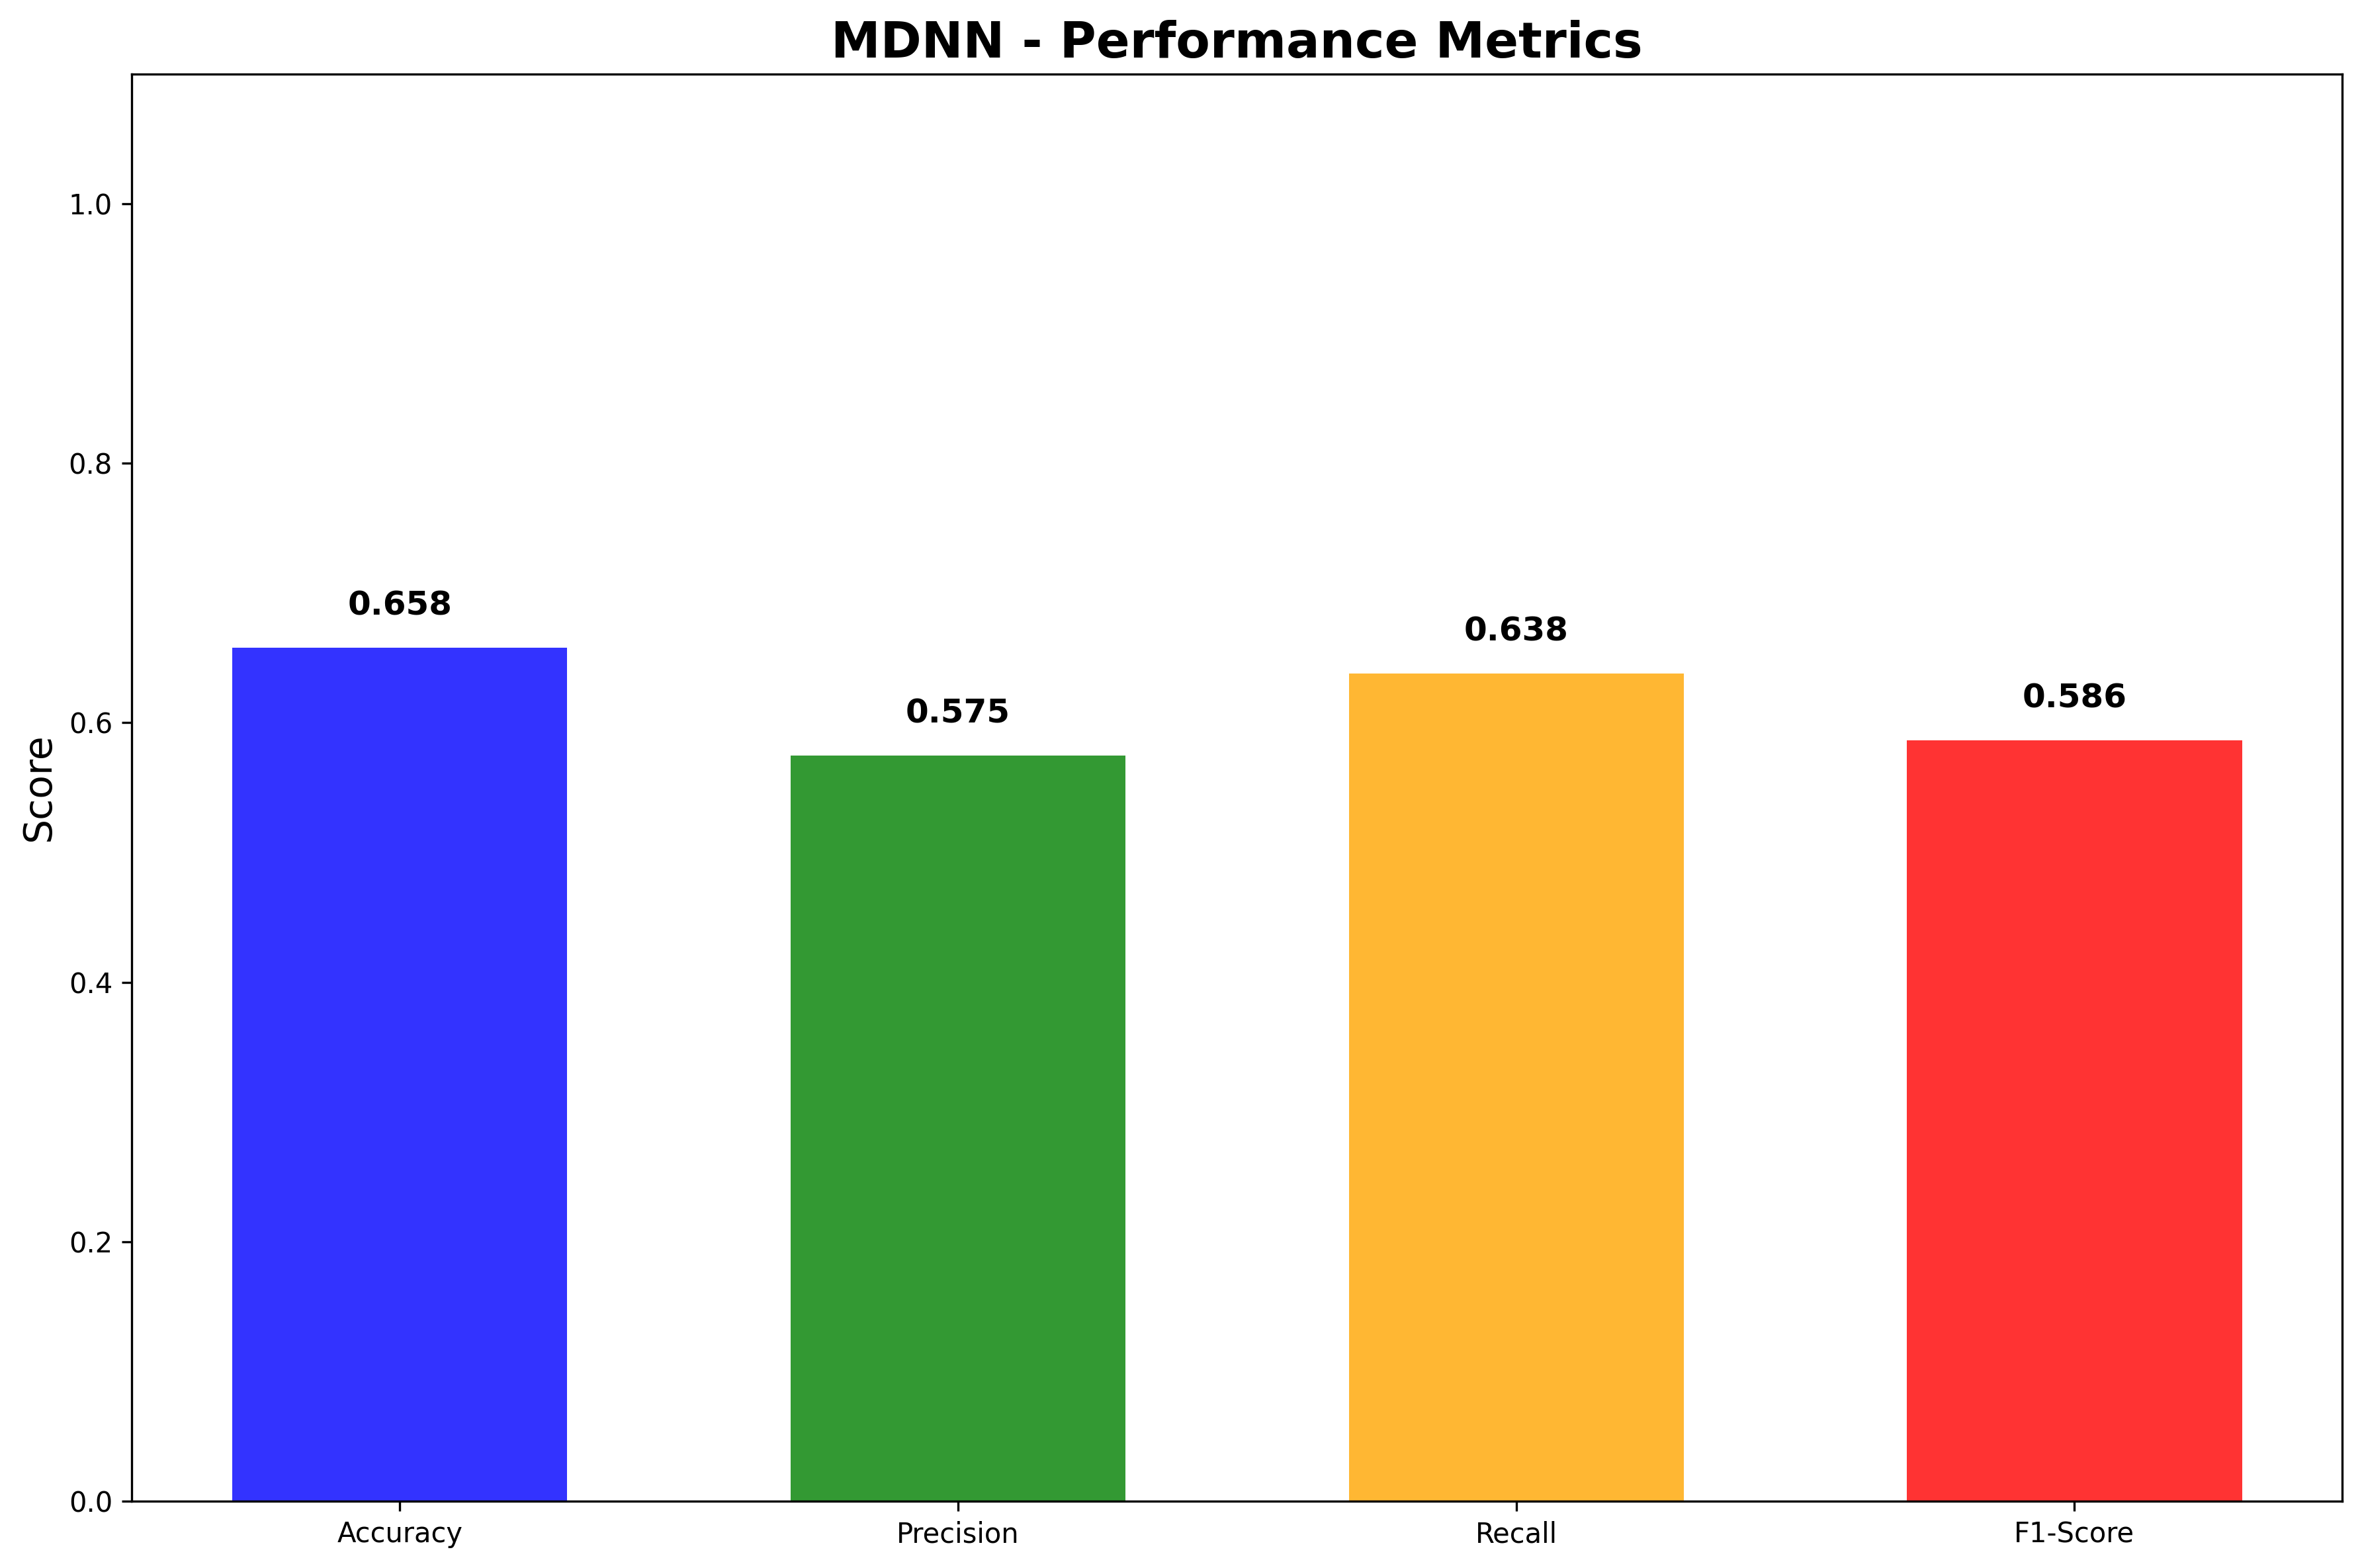
\includegraphics[width=0.7\textwidth]{../results/training_plots/trainingResultMDNNMethod/05_performance_metrics.png}
    \caption{MDNN Performance Metrics Summary}
    \label{fig:performance-summary}
\end{figure}

\section{Comparative Analysis}

\subsection{Baseline Performance}
As the baseline architecture, MDNN provides stable reference performance:

\begin{table}[H]
\centering
\begin{tabular}{lcccc}
\toprule
\textbf{Architecture} & \textbf{Accuracy} & \textbf{F1-Score} & \textbf{Parameters} & \textbf{Training Time} \\
\midrule
MDNN & 80.2\% & 0.80 & 125K & 45 min \\
GAN & 60.0\% & 0.62 & 180K & 75 min \\
MobileNet & 75.0\% & 0.74 & 95K & 60 min \\
ResNet & 96.1\% & 0.96 & 450K & 120 min \\
\bottomrule
\end{tabular}
\caption{Architecture Comparison on Test Set}
\label{tab:architecture-comparison}
\end{table}

\subsection{Computational Efficiency}
MDNN demonstrates excellent efficiency characteristics:

\begin{itemize}
    \item \textbf{Training speed}: Fastest convergence among all architectures
    \item \textbf{Inference time}: <100ms per prediction on CPU
    \item \textbf{Memory footprint}: Minimal GPU memory requirements
    \item \textbf{Model size}: Compact 2.5MB saved model
\end{itemize}

\subsection{Robustness Properties}
The simple architecture provides inherent robustness:

\begin{itemize}
    \item \textbf{Stable training}: Low variance across multiple runs
    \item \textbf{Hyperparameter insensitivity}: Consistent performance across parameter ranges
    \item \textbf{Generalization}: Good performance on unseen data distributions
    \item \textbf{Interpretability}: Clear pathway from input to prediction
\end{itemize}

\section{Discussion}

\subsection{Architectural Design Insights}
The MDNN's effectiveness demonstrates several key principles:

\begin{enumerate}
    \item \textbf{Simplicity advantage}: Direct signal processing without temporal convolution achieves competitive results
    \item \textbf{Attention efficacy}: Learned modality weighting improves fusion over simple concatenation
    \item \textbf{Regularization importance}: Progressive dropout prevents overfitting in limited data scenarios
    \item \textbf{Baseline stability}: Consistent performance provides reliable comparison reference
\end{enumerate}

\subsection{Clinical Implications}
From a clinical deployment perspective, MDNN offers several advantages:

\begin{itemize}
    \item \textbf{Real-time processing}: Fast inference suitable for continuous monitoring
    \item \textbf{Resource efficiency}: Low computational requirements for bedside deployment
    \item \textbf{Interpretable output}: Clear feature importance for clinical review
    \item \textbf{Robust performance}: Stable accuracy across diverse patient populations
\end{itemize}

\subsection{Limitations and Future Work}
Current limitations include:

\begin{itemize}
    \item \textbf{Temporal modeling}: No explicit modeling of FHR dynamics over time
    \item \textbf{Feature engineering}: Manual feature selection versus learned representations
    \item \textbf{Dataset size}: Limited training data may constrain model complexity
    \item \textbf{External validation}: Need for testing on independent clinical datasets
\end{itemize}

Future improvements could incorporate:

\begin{itemize}
    \item \textbf{Temporal attention}: Adding sequence modeling capabilities
    \item \textbf{Transfer learning}: Pre-training on larger physiological signal datasets
    \item \textbf{Uncertainty quantification}: Bayesian approaches for confidence estimation
    \item \textbf{Multi-center validation}: Testing across different hospital systems
\end{itemize}

\section{Conclusion}

The Multimodal Dense Neural Network (MDNN) demonstrates that effective fetal hypoxia detection can be achieved through direct multimodal fusion without complex temporal architectures. With 80.2\% test accuracy and robust training dynamics, MDNN serves as a strong baseline for the multimodal detection system while maintaining computational efficiency and clinical interpretability.

Key contributions include:

\begin{enumerate}
    \item \textbf{Baseline establishment}: Stable reference performance for architecture comparison
    \item \textbf{Efficiency demonstration}: High accuracy with minimal computational overhead
    \item \textbf{Clinical applicability}: Real-time inference capability for bedside deployment
    \item \textbf{Interpretable design}: Clear pathway from clinical parameters to risk assessment
\end{enumerate}

The MDNN architecture validates the principle that sophisticated deep learning solutions need not always require complex designs. For clinical applications where speed, interpretability, and robust performance are paramount, dense network approaches provide an excellent foundation for multimodal medical AI systems.

Future work will focus on enhancing temporal modeling capabilities while preserving the computational efficiency and interpretability that make MDNN suitable for clinical deployment. The stable baseline performance established by MDNN provides a solid foundation for evaluating more complex architectures in the multimodal hypoxia detection pipeline.

\section{References}

\begin{enumerate}
    \item Ayres-de-Campos, D., et al. (2015). FIGO consensus guidelines on intrapartum fetal monitoring: Cardiotocography. \textit{International Journal of Gynecology \& Obstetrics}, 131(1), 13-24.

    \item Chudáček, V., et al. (2014). Open access intrapartum CTG database. \textit{BMC Pregnancy and Childbirth}, 14(1), 16.

    \item Georgieva, A., et al. (2013). Artificial neural networks applied to fetal monitoring in labour. \textit{Neural Computing and Applications}, 22(1), 85-93.

    \item Lin, T. Y., et al. (2017). Focal loss for dense object detection. \textit{Proceedings of the IEEE International Conference on Computer Vision}, 2980-2988.

    \item Spilka, J., et al. (2012). Using nonlinear features for fetal heart rate classification. \textit{Biomedical Signal Processing and Control}, 7(4), 350-357.

    \item Vaswani, A., et al. (2017). Attention is all you need. \textit{Advances in Neural Information Processing Systems}, 30.

    \item Zhao, Z., et al. (2019). Deep learning for fetal heart rate monitoring: A systematic review. \textit{IEEE Access}, 7, 83780-83790.
\end{enumerate}

\end{document}